\documentclass[10pt, compress]{beamer}

\usetheme{m}

\usepackage{booktabs}
\usepackage[scale=2]{ccicons}
\usepackage{minted}
\usepackage{tikz}
\usepackage[ruled,vlined,english]{algorithm2e}
\usetikzlibrary{arrows,automata,shapes,positioning,calc}

\newenvironment{exemple}
{\begin{exampleblock}{Exemple}}
{\end{exampleblock}}

\newenvironment{defi}
{\begin{block}{Définition}}
{\end{block}}

\newcommand{\N}[1]{\left\|#1\right\|_2}


\usepgfplotslibrary{dateplot}

\usemintedstyle{trac}

\title{Projet Pensées Profondes}
\subtitle{}
\date{December 18, 2014}
\institute{École Normale Supérieure de Lyon}

\begin{document}

\maketitle

\begin{frame}[fragile]
Raphaël \textsc{Charrondière}

Marc \textsc{Chevalier}

Quentin \textsc{Cormier}

Tom \textsc{Cornebize}

Yassine \textsc{Hamoudi}

Valentin \textsc{Lorentz}

Thomas \textsc{Pellissier} \textsc{Tanon}

\alert{Adviser:} Eddy \textsc{Caron}
\end{frame}

\begin{frame}
    \frametitle{On cherche des réponses}
    \alert{Who was the wife of Louis Pasteur?}
    \begin{figure}
        \includegraphics[width=\textwidth]{pasteurWiki.png}
    \end{figure}
\end{frame}

\begin{frame}
    \frametitle{Outils existants}
    \begin{tabular}{ll}
        WolframAlpha & Marie Pasteur\\
        Google & Article Wikipedia sur Marie Pasteur\\
        Bing & Article Wikipedia Louis Pasteur\\
        Yahoo & Page d'answers.com contenant la question
    \end{tabular}
\medbreak
\alert{Logiciels propriétaire, parfois mauvais...}
\end{frame}

\begin{frame}
    \frametitle{Platypus}
    \begin{center}
        \url{http://askplatyp.us}
        
        \bigskip
        
        \includegraphics[width=0.6\linewidth]{figures/platypus.pdf}
    \end{center}
\end{frame}

\begin{frame}
    \frametitle{Platypus ?}
    \begin{itemize}
        \item<1-> \alert{Open-source}
        \item<2-> \alert{Modulaire}
        \item<3-> \alert{Anglais} pour l'instant
        \item<4-> \alert{Connaissance générale} et math
    \end{itemize}
\end{frame}

\begin{frame}
    \begin{center}
        \Huge Et la démo !
    \end{center}
\end{frame}

\begin{frame}[plain]
    \includegraphics[width=\linewidth]{figures/demo-whoIsAlanTuring.png}
\end{frame}

\begin{frame}[plain]
    \includegraphics[width=\linewidth]{figures/demo-whenIsAlanTuringBorn.png}
\end{frame}

\begin{frame}[plain]
    \includegraphics[width=\linewidth]{figures/demo-whereIsEnsLyon.png}
\end{frame}


\section{Overview}
\begin{frame}[fragile]
    \frametitle{Architecture}
    \begin{figure}
        \includegraphics[scale=.21]{figures/architecture}
    \end{figure}
\end{frame}

\begin{frame}
  \frametitle{Une question}
    \alert{Where does the prime minister of the United Kingdom live?}
\end{frame}

\begin{frame}
 \frametitle{De la question à la forme normale}

\begin{center}
  \alert{Where does the prime minister of the United Kingdom live?}
\end{center}

\begin{figure}
 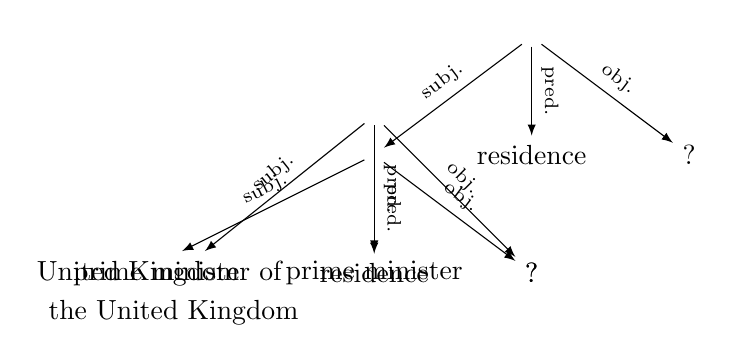
\begin{tikzpicture}
  \onslide<1>{
  \node (7) at (8,9) {$\triple$};
  \node (8) at (5.5,7) {prime minister of};
  \node (11) at (5.45,6.5) {the United Kingdom};
  \node (9) at (8,7) {residence};
  \node (10) at (10,7) {?};

  \draw[->, >=latex] (7) edge node[sloped, anchor=center, above] {\scriptsize{subj.}} (8);
  \draw[->, >=latex] (7) edge node[sloped, anchor=center, above] {\scriptsize{pred.}} (9);
  \draw[->, >=latex] (7) edge node[sloped, anchor=center, above] {\scriptsize{obj.}} (10);}
  
  \onslide<2>{  
  \node (0) at (10,10) {$\triple$};
  \node (1) at (10,8.5) {residence};
  \node (2) at (12,8.5) {?};
  \node (3) at (8,8.5) {$\triple$};
  \node (4) at (8,7) {prime minister};
  \node (5) at (5,7) {United Kingdom};
  \node (6) at (10,7) {?};

  \draw[->, >=latex] (0) edge node[sloped, anchor=center, above] {\scriptsize{obj.}} (2);
  \draw[->, >=latex] (0) edge node[sloped, anchor=center, above] {\scriptsize{pred.}} (1);
  \draw[->, >=latex] (0) edge node[sloped, anchor=center, above] {\scriptsize{subj.}} (3);
  \draw[->, >=latex] (3) edge node[sloped, anchor=center, above] {\scriptsize{subj.}} (5);
  \draw[->, >=latex] (3) edge node[sloped, anchor=center, above] {\scriptsize{obj.}} (6);
  \draw[->, >=latex] (3) edge node[sloped, anchor=center, above] {\scriptsize{pred.}} (4);}
 \end{tikzpicture}
\end{figure}

\end{frame}

\begin{frame}
   \frametitle{Extraction de la réponse : Wikidata}

    Wikidata ?
    \begin{itemize}
        \item \alert{\url{http://www.wikidata.org}}
        \item Une base de \alert{connaissance libre}
        \item \alert{Multilingue}
    \end{itemize}
\end{frame}

\begin{frame}
  \frametitle{Extraction de la réponse : Wikidata}

\begin{figure}
 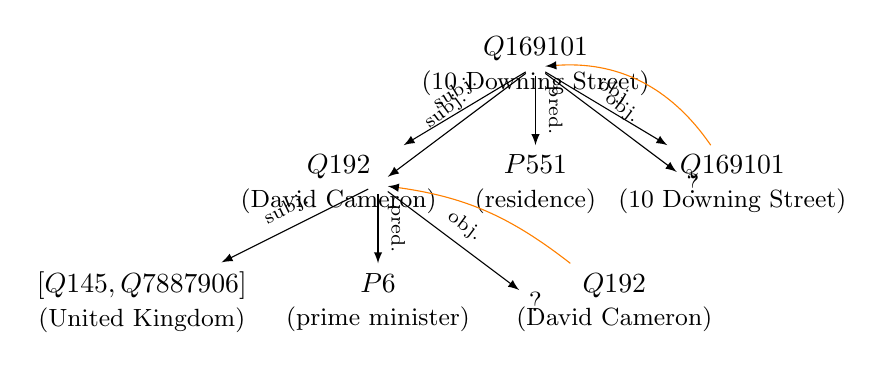
\begin{tikzpicture}
  \onslide<1-4>{\node (0) at (10,10) {$\triple$};}
  \onslide<1-4>{\node (1) at (10,8.5) [align=center] {$P551$\\{\small (residence)}};}
  \onslide<1-3>{\node (2) at (12,8.5) {?};}
  \onslide<1-2>{\node (3) at (8,8.5) {$\triple$};}
  \onslide<1-2>{\node (4) at (8,7) [align=center] {$P6$\\{\small (prime minister)}};}
  \onslide<1-2>{\node (5) at (5,7) [align=center] {$\left[Q145, Q7887906\right]$\\{\small (United Kingdom)}};}
  \onslide<1>{\node (6) at (10,7) {?};}

  \onslide<1-4>{\draw[->, >=latex] (0) edge node[sloped, anchor=center, above] {\scriptsize{pred.}} (1);}
  \onslide<1-3>{\draw[->, >=latex] (0) edge node[sloped, anchor=center, above] {\scriptsize{obj.}} (2);}
  \onslide<1-2>{\draw[->, >=latex] (0) edge node[sloped, anchor=center, above] {\scriptsize{subj.}} (3);}
  \onslide<1-2>{\draw[->, >=latex] (3) edge node[sloped, anchor=center, above] {\scriptsize{subj.}} (5);}
  \onslide<1-2>{\draw[->, >=latex] (3) edge node[sloped, anchor=center, above] {\scriptsize{obj.}} (6);}
  \onslide<1-2>{\draw[->, >=latex] (3) edge node[sloped, anchor=center, above] {\scriptsize{pred.}} (4);}
  
  \onslide<2>{\node (7) at (11,7) [align=center] {\alert{$Q192$}\\\alert{\small (David Cameron)}};}
  \onslide<3-4>{\node (8) at (7.5,8.5) [align=center] {\alert{$Q192$}\\\alert{\small (David Cameron)}};}
  \onslide<4>{\node (9) at (12.5,8.5) [align=center] {\alert{$Q169101$}\\\alert{\small (10 Downing Street)}};}
  \onslide<5>{\node (10) at (10,10) [align=center] {\alert{$Q169101$}\\\alert{\small (10 Downing Street)}};}

  \onslide<3-4>{\draw[->, >=latex] (0) edge node[sloped, anchor=center, above] {\scriptsize{subj.}} (8);}
  \onslide<4>{\draw[->, >=latex] (0) edge node[sloped, anchor=center, above] {\scriptsize{obj.}} (9);}

  \onslide<2>{\draw[->, >=latex] [draw=orange] [bend right=15, above] (7) edge (3);}
  \onslide<4>{\draw[->, >=latex] [draw=orange] [bend right, above] (9) edge (0);}
 \end{tikzpicture}
\end{figure}
\end{frame}


\begin{frame}
    \frametitle{Résultat final}
    \includegraphics[width=\linewidth]{figures/residence-prime-minister.png}
\end{frame}

\begin{frame}
    \frametitle{Recherche simple}
    \includegraphics[width=\linewidth]{figures/10-downing-street.png}
\end{frame}

\begin{frame}
    \frametitle{Math}
    TODO
\end{frame}


\section{Question parsing}

\subsection{Grammatical approach}

%#############################################################################################################%
%#############################################################################################################%
\iffalse
\begin{frame}[fragile]
  \frametitle{Example}

\begin{center}
  \alert{Where does the prime minister of United Kingdom live?}
\end{center}

\end{frame}
\fi
%#############################################################################################################%
%#############################################################################################################%

\begin{frame}[fragile]
  \frametitle{Dependency tree output by the Stanford Parser}

\begin{figure}
\begin{tikzpicture}
  \node (0) at (10,10) {ROOT};
  \node (1) at (10,8.5) {live};
  \node (2) at (8,7) {minister};
  \node (3) at (10,7) {does};
  \node (4) at (12,7) {Where};
  \node (5) at (6,5.5) {the};
  \node (6) at (8,5.5) {prime};
  \node (7) at (10,5.5) {Kingdom};
  \node (8) at (10,4) {United};

  \node (9) at (14,1) {}; % utilisé pour forcer le positionnement de la figure globale

  \draw[->, >=latex] (0) edge node[anchor=center, right] {\scriptsize{root}} (1);
  \draw[->, >=latex] (1) edge node[anchor=center, left] {\scriptsize{nsubj}} (2);
  \draw[->, >=latex] (1) edge node[anchor=center, right] {\scriptsize{aux}} (3);
  \draw[->, >=latex] (1) edge node[anchor=center, right] {\scriptsize{advmod}} (4);
  \draw[->, >=latex] (2) edge node[anchor=center, left] {\scriptsize{det}} (5);
  \draw[->, >=latex] (2) edge node[anchor=center, right] {\scriptsize{prep\_of}} (7);
  \draw[->, >=latex] (2) edge node[anchor=center, left] {\scriptsize{amod}} (6);
  \draw[->, >=latex] (7) edge node[anchor=center, right] {\scriptsize{nn}} (8);
 \end{tikzpicture}
\end{figure}

\end{frame}

%#############################################################################################################%
%#############################################################################################################%

\begin{frame}[fragile]
  \frametitle{Identify question word}

\begin{figure}
 \begin{tikzpicture}
  \node (0) at (10,10) {ROOT};
  \node (1) at (10,8.5) {live};
  \node (2) at (8,7) {minister};
  \node (3) at (10,7) {does};
  \onslide<1>{\node (4) at (12,7) {Where};}
  \node (5) at (6,5.5) {the};
  \node (6) at (8,5.5) {prime};
  \node (7) at (10,5.5) {Kingdom};
  \node (8) at (10,4) {United};
  
  \node (9) at (14,1) {}; % utilisé pour forcer le positionnement de la figure globale

  \onslide<1>{\draw [draw=orange] (11.4,7.2) rectangle (12.6,6.8);}
  \onslide<1>{\node (9) at (13,6.5) {\footnotesize{Question word}};}
  
  \draw[->, >=latex] (0) edge node[anchor=center, right] {\scriptsize{root}} (1);
  \draw[->, >=latex] (1) edge node[anchor=center, left] {\scriptsize{nsubj}} (2);
  \draw[->, >=latex] (1) edge node[anchor=center, right] {\scriptsize{aux}} (3);
  \onslide<1>{\draw[->, >=latex] (1) edge node[anchor=center, right] {\scriptsize{advmod}} (4);}
  \draw[->, >=latex] (2) edge node[anchor=center, left] {\scriptsize{det}} (5);
  \draw[->, >=latex] (2) edge node[anchor=center, right] {\scriptsize{prep\_of}} (7);
  \draw[->, >=latex] (2) edge node[anchor=center, left] {\scriptsize{amod}} (6);
  \draw[->, >=latex] (7) edge node[anchor=center, right] {\scriptsize{nn}} (8);
  
  \onslide<2->{}
 \end{tikzpicture}
\end{figure}
  
\end{frame}

%#############################################################################################################%
%#############################################################################################################%

\begin{frame}[fragile]
  \frametitle{Merging}

\begin{figure}
 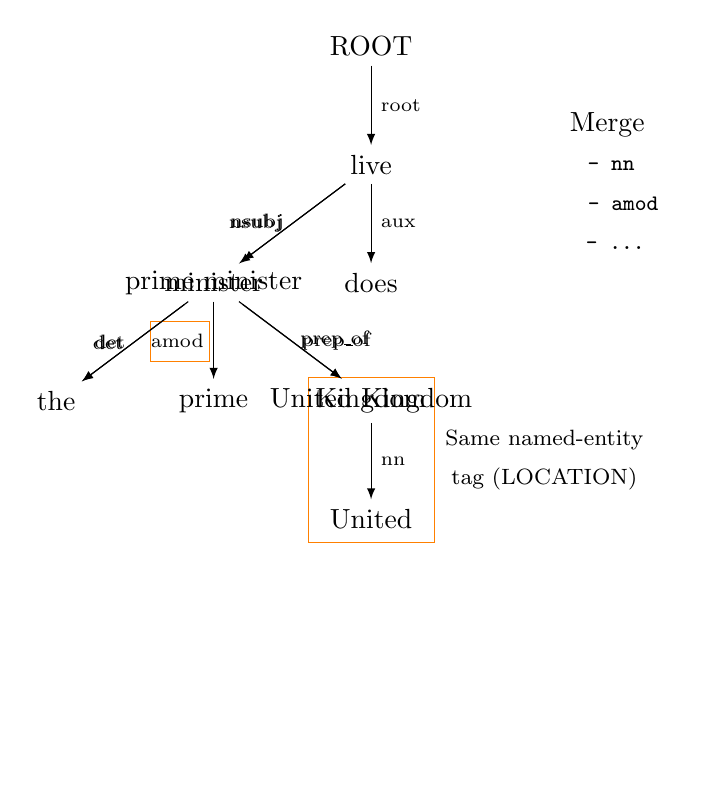
\begin{tikzpicture}
  \node (0) at (10,10) {ROOT};
  \node (1) at (10,8.5) {live};
  \onslide<-3>{\node (2) at (8,7) {minister};}
  \node (3) at (10,7) {does};
  \node (5) at (6,5.5) {the};
  \onslide<-3>{\node (6) at (8,5.5) {prime};}
  \onslide<1>{\node (7) at (10,5.5) {Kingdom};}
  \onslide<1>{\node (8) at (10,4) {United};}

  \node (9) at (14,1) {}; % utilisé pour forcer le positionnement de la figure globale

  \onslide<1>{\draw [draw=orange] (9.2,5.8) rectangle (10.8,3.7);}
  \onslide<1>{\node (10) at (12.2,5) {\footnotesize{Same named-entity}};}
  \onslide<1>{\node (11) at (12.2,4.5) {\footnotesize{tag (\alert{LOCATION})}};}

  \onslide<2->{\node (12) at (10,5.5) {United Kingdom};}

  \draw[->, >=latex] (0) edge node[anchor=center, right] {\scriptsize{root}} (1);
  \onslide<-3>{\draw[->, >=latex] (1) edge node[anchor=center, left] {\scriptsize{nsubj}} (2);}
  \draw[->, >=latex] (1) edge node[anchor=center, right] {\scriptsize{aux}} (3);
  \onslide<-3>{\draw[->, >=latex] (2) edge node[anchor=center, left] {\scriptsize{det}} (5);}
  \onslide<-3>{\draw[->, >=latex] (2) edge node[anchor=center, right] {\scriptsize{prep\_of}} (7);}
  \onslide<-3>{\draw[->, >=latex] (2) edge node[anchor=center, left] {\scriptsize{amod}} (6);}
  \onslide<1>{\draw[->, >=latex] (7) edge node[anchor=center, right] {\scriptsize{nn}} (8);}
  
  % fusion du amod
  
  \onslide<3>{\draw [draw=orange] (7.2,6.5) rectangle (7.95,6);}
  
  \onslide<3,4>{
  \node (13) at (13,9) {\alert{Merge}};
  \node (14) at (13.05,8.5) {\footnotesize{\texttt{- nn}}}; 
  \node (15) at (13.2,8) {\footnotesize{\texttt{- amod}}}; 
  \node (16) at (13.1,7.5) {\footnotesize{\texttt{- ...}}};}

  \onslide<4->{\node (17) at (8,7) {prime minister};}
  \onslide<4>{\draw[->, >=latex] (1) edge node[anchor=center, left] {\scriptsize{nsubj}} (17);}
  \onslide<4>{\draw[->, >=latex] (17) edge node[anchor=center, right] {\scriptsize{prep\_of}} (7);}
  \onslide<4>{\draw[->, >=latex] (17) edge node[anchor=center, left] {\scriptsize{det}} (5);}
  \end{tikzpicture}
\end{figure}
  
\end{frame}

%#############################################################################################################%
%#############################################################################################################%

\begin{frame}[fragile]
  \frametitle{Removal}

\begin{figure}
 \begin{tikzpicture}
  \node (0) at (10,10) {ROOT};
  \node (1) at (10,8.5) {live};
  \node (2) at (8,7) {prime minister};
  \onslide<1>{\node (3) at (10,7) {does};}
  \onslide<1>{\node (5) at (6,5.5) {the};}
  \node (7) at (10,5.5) {United Kingdom};

  \node (8) at (14,1) {}; % utilisé pour forcer le positionnement de la figure globale

  \onslide<1>{\draw [draw=orange] (6.4,6.5) rectangle (7,5.9);}
  \onslide<1>{\draw [draw=orange] (10.05,7.9) rectangle (10.6,7.6);}
  
  \node (9) at (13,9) {\alert{Remove}};
  \node (10) at (13.1,8.5) {\footnotesize{\texttt{- det}}}; 
  \node (11) at (13.1,8) {\footnotesize{\texttt{- aux}}}; 
  \node (12) at (13.1,7.5) {\footnotesize{\texttt{- ...}}};
  
  \draw[->, >=latex] (0) edge node[anchor=center, right] {\scriptsize{root}} (1);
  \draw[->, >=latex] (1) edge node[anchor=center, left] {\scriptsize{nsubj}} (2);
  \onslide<1>{\draw[->, >=latex] (1) edge node[anchor=center, right] {\scriptsize{aux}} (3);}
  \onslide<1>{\draw[->, >=latex] (2) edge node[anchor=center, left] {\scriptsize{det}} (5);}
  \draw[->, >=latex] (2) edge node[anchor=center, right] {\scriptsize{prep\_of}} (7);

  \onslide<2>{} % forcer slide 2
  \end{tikzpicture}
\end{figure}
  
\end{frame}


%#############################################################################################################%
%#############################################################################################################%

\begin{frame}[fragile]
  \frametitle{Nounification}

\begin{figure}
 \begin{tikzpicture}
  \node (0) at (10,10) {ROOT};
  \onslide<1>{\node (1) at (10,8.5) {live};}
  \node (2) at (8,7) {prime minister};
  \node (7) at (10,5.5) {United Kingdom};

  \node (8) at (6.45,1) {}; % utilisé pour forcer le positionnement de la figure globale

  \onslide<1>{\draw[->, >=latex] (0) edge node[anchor=center, right] {\scriptsize{root}} (1);}
  \onslide<1>{\draw[->, >=latex] (1) edge node[anchor=center, left] {\scriptsize{nsubj}} (2);}
  \draw[->, >=latex] (2) edge node[anchor=center, right] {\scriptsize{prep\_of}} (7);
  
  \node (18) at (12.7,9) {\alert{Nounify}};
  \onslide<1>{\draw [draw=orange] (9.6,8.7) rectangle (10.4,8.3);}
  
  \onslide<2->{\node (22) at (10,8.5) {residence};}
  \onslide<2->{\draw[->, >=latex] (0) edge node[anchor=center, right] {\scriptsize{root}} (22);}
  \onslide<2->{\draw[->, >=latex] (22) edge node[anchor=center, left] {\scriptsize{nsubj}} (2);}
  \end{tikzpicture}
\end{figure}
  
\end{frame}

%#############################################################################################################%
%#############################################################################################################%

\begin{frame}[fragile]
  \frametitle{Replacement rules}

\begin{figure}
 \begin{tikzpicture}
  \node (0) at (10,10) {ROOT};
  \node (22) at (10,8.5) {residence};
  \node (2) at (8,7) {prime minister};
  \node (7) at (10,5.5) {United Kingdom};

  \node (8) at (14,1) {}; % utilisé pour forcer le positionnement de la figure globale

  \onslide<1>{\draw[->, >=latex] (0) edge node[anchor=center, right] {\scriptsize{root}} (22);}
  \onslide<1>{\draw[->, >=latex] (22) edge node[anchor=center, left] {\scriptsize{nsubj}} (2);}
  \onslide<1>{\draw[->, >=latex] (2) edge node[anchor=center, right] {\scriptsize{prep\_of}} (7);} 
  
  \onslide<1>{\draw [draw=orange] (10.05,9.5) rectangle (10.7,9);}
  \onslide<1>{\draw [draw=orange] (8.2,8) rectangle (9,7.6);}
  \onslide<1>{\draw [draw=orange] (9,6.5) rectangle (10.1,6);}

  \node (18) at (12.7,9) {\alert{Replace}};
  \node (19) at (14.55,8.5) {\footnotesize{\texttt{- nsubj, prep\_of, ...} $\rightarrow R_5$}}; 
  \node (20) at (14.2,8) {\footnotesize{\texttt{- comp, vmod, ...} $\rightarrow R_3$}}; 
  \node (21) at (12.8,7.5) {\footnotesize{\texttt{- ...}}};

  \onslide<2->{\draw[->, >=latex] (0) edge node[anchor=center, right] {\scriptsize{$R_0$}} (22);}
  \onslide<2->{\draw[->, >=latex] (22) edge node[anchor=center, left] {\scriptsize{$R_5$}} (2);}
  \onslide<2->{\draw[->, >=latex] (2) edge node[anchor=center, right] {\scriptsize{$R_5$}} (7);}
  \end{tikzpicture}
\end{figure}
  
\end{frame}

%#############################################################################################################%
%#############################################################################################################%

\begin{frame}[fragile]
  \frametitle{Normalization}
  
\begin{figure}
 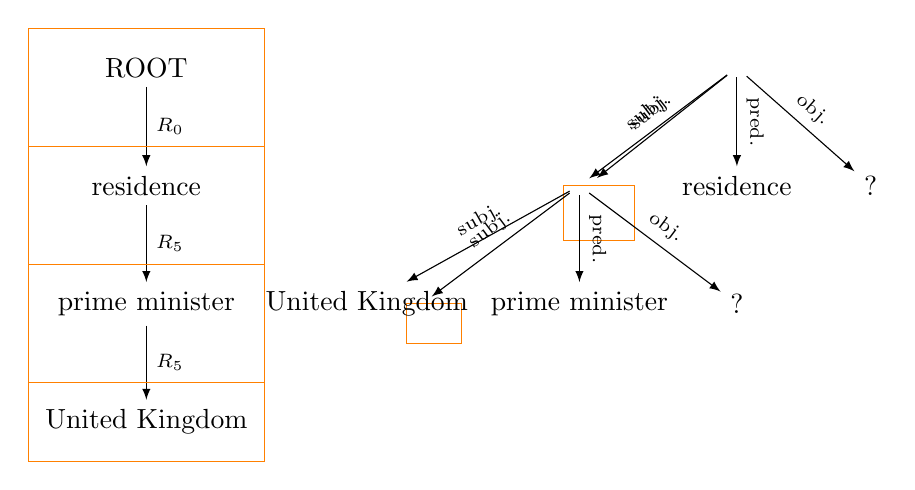
\begin{tikzpicture}
  \node (0) at (9,10) {ROOT};
  \node (1) at (9,8.5) {residence};
  \node (2) at (9,7) {prime minister};
  \node (3) at (9,5.5) {United Kingdom};

  \draw[->, >=latex] (0) edge node[anchor=center, right] {\scriptsize{$R_0$}} (1);
  \draw[->, >=latex] (1) edge node[anchor=center, right] {\scriptsize{$R_5$}} (2);
  \draw[->, >=latex] (2) edge node[anchor=center, right] {\scriptsize{$R_5$}} (3); 
  
  \onslide<1>{\draw [draw=orange] (7.5,10.5) rectangle (10.5,5);}
  \onslide<2>{\draw [draw=orange] (7.5,9) rectangle (10.5,5);}
  \onslide<3>{\draw [draw=orange] (7.5,7.5) rectangle (10.5,5);}
  \onslide<4>{\draw [draw=orange] (7.5,6) rectangle (10.5,5);}

  %%%%
  
  \onslide<3->{
  \node (4) at (16.5,10) {$\triple$};
  \node (5) at (14.6,8.5) {};
  \node (6) at (16.5,8.5) {residence};
  \node (7) at (18.2,8.5) {?};

  \draw[->, >=latex] (4) edge node[sloped, anchor=center, above] {\scriptsize{pred.}} (6);
  \draw[->, >=latex] (4) edge node[sloped, anchor=center, above] {\scriptsize{obj.}} (7); }
  \onslide<3>{\draw[->, >=latex] (4) edge node[sloped, anchor=center, above] {\scriptsize{subj.}} (5);}
  
  \onslide<3>{\draw [draw=orange] (14.3,8.5) rectangle (15.2,7.8);}

  \onslide<4->{
  \node (8) at (14.5,8.5) {$\triple$};
  \node (9) at (12.5,7) {};
  \node (10) at (14.5,7) {prime minister};
  \node (11) at (16.5,7) {?};

  \draw[->, >=latex] (4) edge node[sloped, anchor=center, above] {\scriptsize{subj.}} (8);
  \draw[->, >=latex] (8) edge node[sloped, anchor=center, above] {\scriptsize{pred.}} (10);
  \draw[->, >=latex] (8) edge node[sloped, anchor=center, above] {\scriptsize{obj.}} (11); }

  \onslide<4>{\draw[->, >=latex] (8) edge node[sloped, anchor=center, above] {\scriptsize{subj.}} (9);}

  \onslide<4>{\draw [draw=orange] (12.3,7) rectangle (13,6.5);}
  
  \onslide<5>{\node (12) at (11.8,7) {United Kingdom};
  \draw[->, >=latex] (8) edge node[sloped, anchor=center, above] {\scriptsize{subj.}} (12);}
 \end{tikzpicture}
\end{figure}

\end{frame}

\subsection{Machine Learning \--- Reformulation}

\subsubsection{Aim}

\begin{frame}
\frametitle{Aim}
\alert{Reformulation?}

\pause


((United States, birth date, ?),president, ?)

$\mapsto$

((United States, president, ?),birth date, ?)

%Changing the form, not the content.
\end{frame}

\subsubsection{Operation}
\begin{frame}
\frametitle{Operation}
\alert{Projection:} trees $\mapsto$ vector space.

The dictionary associates a vector triple to a vector.
\end{frame}

\begin{frame}
\frametitle{Projection}
\begin{tikzpicture}[x=2.5cm]
\node (s) at (1,0) {s};
\node (p) at (3,0) {p};
\node (r) at (2,1) {r};


\node (a) at (2,2) {a=compact(s,r,p)};
\node (b) at (4,2) {b};
\node (l) at (3,3) {l};
\node (h) at (3,4) {h=compact(a,l,b)};

\draw (s)--(a)--(p);
\draw (r)--(a);
\draw (a)--(h)--(b);
\draw (l)--(h);
\end{tikzpicture}
\end{frame}

\subsubsection{Build the request}

\begin{frame}
\frametitle{From vector to tree}

\begin{tikzpicture}[x=2.5cm]
\node (s) at (1,0) {s};
\node (p) at (3,0) {p};
\node (r) at (2,0) {r};
\node (sf) at (1,-1) {\textbf{nearest}};
\node (pf) at (3,-1) {\textbf{nearest}};
\node (rf) at (2,-1) {\textbf{nearest}};
\node (sw) at (1,-2) {word};
\node (pw) at (3,-2) {word};
\node (rw) at (2,-2) {word};
\node[rectangle] (b) at (2,2) {\textbf{uncompact}};
\node (a) at (2,3) {v};
%\node (b) at (4,2) {b};
%\node (l) at (3,3) {l};
%\node (h) at (3,4) {h=compact(a,l,b)};

\draw[->, >=latex] (b)--(s);
\draw[->, >=latex] (b)--(p);
\draw[->, >=latex] (b)--(r);
\draw[->, >=latex] (a)--(b);
\draw[->, >=latex] (r)--(rf);
\draw[->, >=latex] (p)--(pf);
\draw[->, >=latex] (s)--(sf);
\draw[->, >=latex] (rf)--(rw);
\draw[->, >=latex] (pf)--(pw);
\draw[->, >=latex] (sf)--(sw);

\draw [->, >=latex] (pf.east)        to [bend right=90] (a);
\draw [->, >=latex] (sf.west)        to [bend left=90] (a);
\end{tikzpicture}

\end{frame}

\subsubsection{Learn}

\begin{frame}
\frametitle{Training}
Semantic distance.

Use relation graph ``instance of'' from Wikidata.
\end{frame} 


\subsection{Machine Learning \--- Standalone}

\begin{frame}[fragile]
  \frametitle{Keywords questions}

	
	\begin{center}
  	\alert{United States president}
	\end{center}

	\begin{center}
  	\alert{president United States}
	\end{center}

\end{frame}

\begin{frame}[fragile]

Classify each word into one of the four categories: \{to ignore, subject, predicate, object \}

\end{frame}

\begin{frame}[fragile]

	\begin{center}
  	\alert{(United, subject) (States, subject) (president, predicate)}
	\end{center}

	\begin{center}
  	\alert{(president, predicate) (United, subject) (States, subject)}
	\end{center}



\end{frame}

\begin{frame}[fragile]
  \frametitle{Look-up table}

	\begin{center}
	Word $w \Rightarrow $ Vector $ V_w \in \mathbb{R}^{25}$
	\end{center}

	\begin{center}
	If two words $w_1$ and $w_2$ are synonymous then, \newline
	$$ || w_2 - w_1 ||_2 \approx 0 $$
	
	\end{center}



\end{frame}





\section{Back-end}

\section{Wikidata}

\subsection{Overview}
Wikidata module\footnote{\url{https://github.com/ProjetPP/PPP-Wikidata/}} is our main proof of concept module which aims to demonstrate the ability of our framework to allow the easy creation of huge modules able to answer thousand of questions. This module tries to answer general knowledge using the data stored in Wikidata\footnote{\url{http://www.wikidata.org/}}.

\begin{figure}[!ht]
  \centering
    \label{wikidata:item-screenshot}
    \includegraphics[width=\textwidth]{./wikidata-item-screenshot.png}
    \caption{The beginning of a Wikidata item}
\end{figure}

Wikidata is a free knowledge base hosted by the Wikimedia Foundation as a sister project of Wikipedia. It aims to build a free, collaborative, multilingual structured database of general knowledge (for more information see \cite{42240}). It provides a very good set of API that allows to consume and query Wikidata content easily. Wikidata is built upon entities (called items and stored in a separated wiki pages) that are about a given subject. Each item has a label, a description and some aliases to describe it and statements that provides data about this subject (see figure \ref{wikidata:item-screenshot}). Each statement is built around a property and a value such that $(item, property, value)$ may be seen as a valid triple. Properties are entities like items and so may have labels, descriptions, aliases and statements. For more information see\footnote{\url{http://www.wikidata.org/wiki/Wikidata:Glossary}}.

We have chosen Wikidata instead of some other famous knowledge base like DBpedia\footnote{\url{http://dbpedia.org}} or Freebase\footnote{\url{http://www.freebase.com/}} because Wikidata is under a CC0 license\footnote{\url{http://creativecommons.org/publicdomain/zero/1.0/}} that allows to reuse data without constraints and is fully multilingual, a characteristic that will be very useful in order to adapt the PPP to other languages than English. More, as one of the members of the team is involved in Wikidata it allows us to avoid to lose time by learning the other knowledge base APIs.

\subsection{APIs}
Wikidata provides an API that allows to retrieve items and properties from there ids and an API that returns items or properties that match a given label. For more information about the API see the appendix \ref{wikidata:api-examples}.

Some libraries are available to interact easily with the API. The two major ones are:
\begin{itemize}
    \item \textbf{Wikidata Toolkit}\footnote{\url{http://www.mediawiki.org/wiki/Wikidata_Toolkit}} written in Java and allows to interact easily with the API and dumps of Wikidata content that are regularly done.
    \item \textbf{wikibase-api}\footnote{\url{https://github.com/addwiki/wikibase-api}} written in PHP that only allows to interact with the API but has the strong advantages to share a lot of code with the MediaWiki extension that powers Wikidata\footnote{\url{https://www.mediawiki.org/wiki/Wikibase}}.
\end{itemize}

We have chosen to use the PHP API because one of the members of the team has contributed in a significant manner to it and so was able to have a working module quickly.

In order to do queries in Wikidata content, like retrieving all presidents of the United States, e.g. all items with the property "position held" (P39) with value "president of the united States of America" (Q11696) we had to rely on an external service, called \textbf{WikidataQuery}\footnote{\url{http://wdq.wmflabs.org/}} that allows to do such requests. This was needed because the Wikidata API does not allow to do such queries yet. We have written a small standalone and reusable wrapper to the API of this service in PHP\footnote{\url{https://github.com/ProjetPP/WikidataQueryApi/}}.

\subsection{Implementation}
In order to write this module nicely we have written a small PHP library, LibModule\url{https://github.com/ProjetPP/PPP-LibModule-PHP}, that provides a framework to create PPP modules and diverse utilities to simplify nodes like union or intersection that do not requires specific knowledge about the resources themselves.

This module works in tree steps:
\begin{enumerate}
    \item It maps \textit{resource} nodes of the question tree into Wikidata content: the subjects of \textit{triple} nodes are mapped to Wikidata items, predicates to Wikidata properties and objects to the type of value that is the range of the Wikidata property of the predicate. If more than one match are possible, a tree per possible match is output.
    \item It performs queries against Wikidata content using the previously done mapping to reduce as much as possible trees. When we have a \textit{triple} node where the object is missing the module gets the Wikidata item of the subject, looks for values for the predicate property and replace the \textit{triple} node with a \textit{resource} node for each value of the triple (and so builds as many trees as there are values). When there is a \textit{triple} node with a missing subject the module uses the WikidataQuery API.
    \item It adds clean representation of \textit{resource} nodes added by the previous phase. When Wikidata resources are returns it keeps their IDs in order to allow the ui to create nice display of them.
\end{enumerate}

We have also added specific support for "name", "definition" and "identity" predicates in order to allows the API to have a nice display of the "Barack Obama" item when the query is "Who is Barack Obama?", rewritten as \textit{(Barack Obama, identity, ?)}. the same thing applies if the module input is a sentence like "Barack Obama".

One of the difficulties met was to avoid meaningless results because Wikidata contains items about Wikipedia organizational content like "disambiguation" or "category" pages. So we have written a small filter that ignore these pages when the conversion string to Wikidata identifier is done.

\begin{figure}[!h]
  \centering
    \label{wikidata:struct}
    \includegraphics[width=\textwidth]{./wikidata_louis13_children.png}
    \caption{An example output from the Wikidata module}
\end{figure}

\subsection{Future work}

This module is only at its first stage and a lot of nice to have features remains:
\begin{itemize}
    \item Clever filter of not relevant results: people that are looking for the list of the presidents of the United States are usually not looking for fictional ones.
    \item Handle triple that does not directly match to Wikidata model. If we looks for people born in France we are also looking for people born in Lyon or if we are looking for the American Secretary of State we are looking for the person that has as office "American Secretary of State".
    \item Do some reasoning on Wikidata content. For example if \texttt{(Lyon, instance of, city)} and \texttt{(city, subclass of, place)} then we should be able to guess and use that \texttt{(Lyon, instance of, place)}.
\end{itemize}


\subsection{Add-ons}

\begin{frame}[fragile]
    \frametitle{Computer Algebra System}
\end{frame}

\begin{frame}[fragile]
    \frametitle{Spell Checker}
    Based on \alert{GNU Aspell}.

    \medbreak

    What are the langajes of Soth Afryka?

    $\rightarrow$

    What are the languages of South Africa?
\end{frame}


\section{Better than Wolfram?}
\subsection{Better than Wolfram?}

\begin{frame}
    \frametitle{Nested question}

Who is the wife of the president of the United States?
    \begin{tabular}{ll}
        \alert{WolframAlpha} & Barack Obama\\
        \alert{Platypus} & Michelle Obama\\
    \end{tabular}

    \medbreak

    \onslide<2->{
        What are the birth dates of the daughters of the wife of the president of the United States?
        \begin{tabular}{ll}
            \alert{WolframAlpha} & Barack Obama\\
            \alert{Platypus} & Saturday, July 4, 1998 \& Sunday, June 10, 2001\\
        \end{tabular}
    }
\end{frame}

\begin{frame}[fragile]
    \frametitle{Conjunction}

Who is the actor of Inception and Titanic?
    \begin{tabular}{ll}
        \alert{WolframAlpha} & all the actors of the two movies\\
        \alert{Platypus} & Leonardo DiCaprio\\
    \end{tabular}
\end{frame}

\subsection{Future work}

\begin{frame}
    \frametitle{Better database}

    ``How fast is the TGV?''

    ``How wide is a tennis court?''

    Not answered by \alert{Wikidata}.

    \medbreak

    $\rightarrow$ Improve Wikidata?

    $\rightarrow$ Use another database?
\end{frame}

\begin{frame}
    \frametitle{Better question parsing}

    ``What is the date of birth of Isaac Newton?''

    ``In which band does Bono sing?''

    Not parsed correctly.

    \medbreak

    $\rightarrow$ Train the Stanford CoreNLP library?

    $\rightarrow$ Improve the algorithm of the Grammatical module?

    $\rightarrow$ Better datasets for the ML modules?
\end{frame}

\begin{frame}
    \frametitle{New modules}
\begin{figure}
 \begin{tikzpicture}
  \node (0) at (-3,2) {\textcolor{mLightBrown}{cooking recipes}};
  \node (0) at (1,1) {\textcolor{mDarkBrown}{HAL}};
  \node (0) at (5,2.5) {\textcolor{mMediumBrown}{meteo}};
  \node (0) at (3,2) {\textcolor{mDarkTeal}{chemistry}};
  \node (0) at (0,0) {\textcolor{mMediumBrown}{programming language interpreter}};
  \node (0) at (-4,-1) {\textcolor{mMediumBrown}{cinema}};
  \node (0) at (0,-2) {\textcolor{mDarkTeal}{music}};
  \node (0) at (4,-1) {\textcolor{mDarkTeal}{literature}};
  \node (0) at (-3,-2) {\textcolor{mDarkBrown}{OEIS}};
  \node (0) at (2,-2.5) {\textcolor{mLightBrown}{translation}};
  \node (0) at (-2,-3) {\textcolor{mMediumBrown}{sport statistics and predictions}};
  \end{tikzpicture}
\end{figure}
\end{frame}

\begin{frame}
    \frametitle{Other ideas...}

    \begin{itemize}
        \item Other languages support (French...)
        \item Improve user experience
        \item Advertise \alert{Platypus}
    \end{itemize}
\end{frame}

\subsection{Conclusion}

\begin{frame}
    \frametitle{Some facts} % to update just before the presentation
    \alert{23 repositories}

    \begin{tabular}{lll}
        6 & PHP & Wikidata libraries and module\\
        12 & Python & Other modules, core, and libraries\\
        1 & C++ & ML-Reformulation\\
        1 & Shell & Deployment scripts\\
        1 & \LaTeX & This presentation and the report\\
        1 & Markdown & The specification\\
        1 & HTML/CSS/Javascript & The Web User Interface\\
        1 & HTML/CSS & The project's website\\
    \end{tabular}

    \alert{1982 commits} (without the ``integration'' repository, which has an automatic commit every 12h)

    \alert{26k lines} of code (13k in PHP, 10k in Python)
\end{frame}

\begin{frame}
    \frametitle{The PPP?}

    \begin{itemize}
        \item A powerful question answering framework
        \item Innovative NLP algorithms
        \item A demo, \alert{Platypus}, with general knowledge and math
    \end{itemize}
\end{frame}


\newlength{\logosize}
\setlength{\logosize}{12pt}
\begin{frame}
    \frametitle{The adventure is only starting...}
    \alert{\url{http://projetpp.github.io/}}

    \begin{tabular}{ll}
        \includegraphics[width=\logosize]{Twitter_logo_blue.png} & \href{https://twitter.com/ProjetPP}{https://twitter.com/ProjetPP}\\
        \includegraphics[width=\logosize]{GitHub-Mark-32px.png} &  \href{https://github.com/ProjetPP}{https://github.com/ProjetPP}\\
        \includegraphics[width=\logosize]{ic_email_black_18dp.png} & \href{mailto:ppp@pony.ovh}{ppp@pony.ovh}\\
    \end{tabular}
\end{frame}


\begin{frame}
    \frametitle{Questions?}
    \begin{center}
        \includegraphics[height=0.7\textheight]{figures/Ornithorhynchus.jpg}
    \end{center}
\end{frame}

\begin{frame}
    \tikzset{
        workpackage/.style={
               node distance = 0.5cm,
               },
    }
    \frametitle{WorkPackages}
    \begin{figure}
        \begin{tikzpicture}
            % PPP members
            \node (rc)                  {Raphaël \textsc{Charrondière}};
            \node (qc)  [below of = rc] {Quentin \textsc{Cormier}};
            \node (tc)  [below of = qc] {Tom \textsc{Cornebize}};
            \node (yh)  [below of = tc] {Yassine \textsc{Hamoudi}};
            \node (mc)  [below of = yh] {Marc \textsc{Chevalier}};
            \node (vl)  [below of = mc] {Valentin \textsc{Lorentz}};
            \node (tpt) [below of = vl] {Thomas \textsc{Pellissier} \textsc{Tanon}};

            % PPP WorkPackages
            \node (reformulation)   [workpackage, right of = rc, right=3cm]  {Reformulation};
            \node (standalone)      [workpackage, below of = reformulation]  {Standalone};
            \node (spellchecker)    [workpackage, below of = standalone]     {SpellChecker};
            \node (communication)   [workpackage, below of = spellchecker]   {Communication};
            \node (grammatical)     [workpackage, below of = communication]  {Grammatical};
            \node (bibliography)    [workpackage, below of = grammatical]    {Bibliography};
            \node (cas)             [workpackage, below of = bibliography]   {CAS};
            \node (datamodel)       [workpackage, below of = cas]            {DataModel};
            \node (architecture)    [workpackage, below of = datamodel]      {Architecture};
            \node (core)            [workpackage, below of = architecture]   {Core};
            \node (sysadmin)        [workpackage, below of = core]           {System Administration};
            \node (wikidata)        [workpackage, below of = sysadmin]       {Wikidata};
            \node (webui)           [workpackage, below of = wikidata]       {WebUI};

            % Edges
            \path (reformulation.west)   edge (rc.east)
                  (standalone.west)      edge (qc.east)
                  (spellchecker.west)    edge (tc.east)
                  (communication.west)   edge (tc.east)
                  (grammatical.west)     edge (tc.east)
                  (grammatical.west)     edge (yh.east)
                  (bibliography.west)    edge (yh.east)
                  (datamodel.west)       edge (yh.east)
                  (datamodel.west)       edge (mc.east)
                  (datamodel.west)       edge (vl.east)
                  (datamodel.west)       edge (tpt.east)
                  (architecture.west)    edge (mc.east)
                  (architecture.west)    edge (vl.east)
                  (architecture.west)    edge (tpt.east)
                  (cas.west)             edge (mc.east)
                  (core.west)            edge (vl.east)
                  (sysadmin.west)        edge (vl.east)
                  (wikidata.west)        edge (vl.east)
                  (wikidata.west)        edge (tpt.east)
                  (webui.west)           edge (tpt.east);
        \end{tikzpicture}
    \end{figure}
\end{frame}


\plain{Questions?}

\end{document}
